\documentclass[10pt]{article}
\usepackage[utf8]{inputenc}	% Para caracteres en español
\usepackage{amsmath,amsthm,amsfonts,amssymb,amscd}
\usepackage{multirow,booktabs}
\usepackage[table]{xcolor}
\usepackage{fullpage}
\usepackage{lastpage}
\usepackage{enumitem}
\usepackage{fancyhdr}
\usepackage{mathrsfs}
\usepackage{wrapfig}
\usepackage{setspace}
\usepackage{calc}
\usepackage{multicol}
\usepackage{cancel}
\usepackage[retainorgcmds]{IEEEtrantools}
\usepackage[margin=3cm]{geometry}
\usepackage{amsmath}
\newlength{\tabcont}
\setlength{\parindent}{0.0in}
\setlength{\parskip}{0.05in}
\usepackage{empheq}
\usepackage{framed}
\usepackage[most]{tcolorbox}
\usepackage{xcolor}
\usepackage{float}
\usepackage[english]{babel}
\usepackage[utf8]{inputenc}
\usepackage{graphicx}
\usepackage[colorinlistoftodos]{todonotes}
\usepackage[version=4]{mhchem}
\usepackage{physics}
\usepackage{mathtools}
%\DeclarePairedDelimiter\bra{\langle}{\rvert}
%\DeclarePairedDelimiter\ket{\lvert}{\rangle}
%\DeclarePairedDelimiterX\braket[2]{\langle}{\rangle}{#1 \delimsize\vert #2}
%\definecolor{shadecolor}{named}{red!25!green!50!blue!75}
\colorlet{NextBlue}{red!25!green!50!blue!75}
%\colorlet{shadecolor}{orange!15}
\colorlet{shadecolor}{NextBlue!40}
\parindent 0in
\parskip 10pt
\geometry{margin=1in, headsep=0.25in}
\theoremstyle{definition}
\newtheorem{defn}{Definition}
\newtheorem{reg}{Rule}
\newtheorem{exer}{Exercise}
\newtheorem{note}{Note}
\begin{document}
\setcounter{section}{1}
\title{Interaction by particle exchange}

%==============================================================
\pagestyle{fancy}
\fancyhf{}
\rhead{Physics 180}
\chead{Interaction by particle exchange}
\lhead{Olyn D. Desabelle}
\rfoot{Page \thepage}
\setlength{\headheight}{12.0pt}

\begin{center}
{\LARGE \bf Interaction by particle exchange}\\
%{\large Physics 170}\\
%Olyn D. Desabelle
\end{center}

\section*{Feynman diagrams}

\begin{figure}[H]
    \centering
    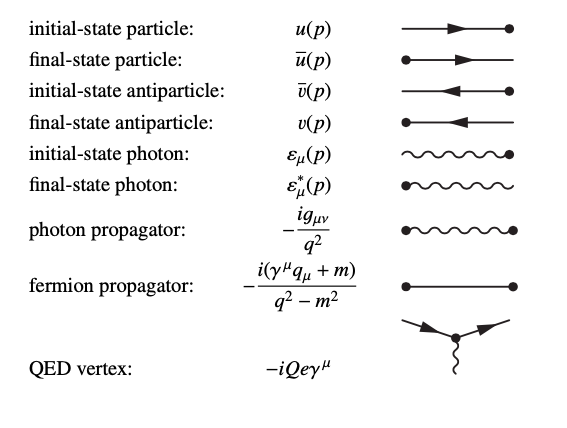
\includegraphics[scale=0.5]{feynman diagram matrix components.png}
\end{figure}

%----------------------------------------

%\subsection*{Dilute Interacting Bose gas}


%----------------------------------------
\end{document}